\chapter{Производительность оборудования и методы ее повышения в оборудовании с ЧПУ} \label{chapt2}

\section{Понятие производительности оборудования} \label{sect2_1}

Современные высокопроизводительные станки с ЧПУ являются довольно дорогим оборудованием, которое зачастую используется на производственных участках неэффективно. Целесообразность использования универсальных обрабатывающих центров вместо узкоспециализированных станков на предприятиях массового и крупносерийного производства обуславливается повышением требований к качеству изделий, необходимостью создавать уникальные и сложные детали с комплексными поверхностями и снижение издержек на производство \cite{Molchanov}. Крупное предприятие может себе позволить закупать подобное оборудование, однако оно требует персонала более высокой квалификации и будет дольше окупаться. Строго говоря, в этом случае есть выбор: рискнуть и вложиться в более универсальное оборудование в целях повышения технико-экономических показателей производства или же заниматься организацией производственных линий на узкоспециализированном оборудовании. В то же время, у малых предприятий такой возможности нет, для них целесообразнее будет использовать универсальное оборудование, исполняющее самые разные техпроцессы изделий.

Одна из проблем оборудования с ЧПУ --- это отсутствие фактического показателя его производительности. В условиях сильного разброса номенклатуры производимых изделий, сложно подсчитать, сколько изделий в единицу времени способно выдать оборудование или производственная линия. Обычно малые предприятия не ведут подобные расчёты, поскольку с малыми тиражами изделий это не имеет смысла. Выполняется изготовление прототипа изделия и далее это время принимается за эталон, который затем умножается на размер партии.

Под производительностью в отношении производства обычно понимается так называемая <<штучная производительность>> --- количество произведённых изделий за единицу времени. Данная величина обратна <<штучному времени>>. Показатель производительности оборудования относится больше к экономическому типу параметров и на крупных предприятиях от его правильного расчёта зависит окупаемость производства. Производительность напрямую относится к показателю эффективности оборудования, которая в литературе носит аббревиатуру OEE (Overall Equipment Effectiveness)\footnote{пер. с англ. --- ``Общая эффективность оборудования''} \cite{Kennet}. Показатель OEE оценивается как произведение трех коэффициентов (\ref{eq_2_1}):

\begin{equation}
OEE = K_{ready} \cdot K_{perf} \cdot K_{qual},
\label{eq_2_1}
\end{equation}

где $K_{ready} = RT / FWT$ --- коэффициент доступности оборудования, то есть, его готовности к работе, он рассчитывается как отношение доступного времени (Ready Time, RT) в единицах времени (например, минутах) к фонду рабочего времени (Fund of Working Time, FTW) в тех же единицах времени; 

$K_{perf} = AP / TP$ --- коэффициент производительности, отражающий отношение фактической производительности (Actual Performance, AP) к теоретической или расчетной (Theoretical Performance, TP), выражаемой в натуральном виде (ед., л., кг и т.д.); 

$K_{qual} = K_{Qprod} / APV$ --- коэффициент качества, отражающий отношение количества бездефектной продукции (вычет процента брака из 100 \%) к объему продукции, произведенной по факту (Actual Product Volume, APV), в натуральном выражении.

Каждая из составляющих OEE характеризуется своими видами потерь при производстве. Так, коэффициент доступности оборудования снижается из-за:

\begin{itemize}
	\item ремонта оборудования (внепланового);
	\item переналадки оборудования;
	\item полного износа или поломки инструмента;
	\item отсутствия готовых материалов для работы;
	\item режима труда и отдыха на предприятии.
\end{itemize}

К потерям в области производительности оборудования можно отнести:

\begin{itemize}
	\item различного рода сбои в оборудовании;
	\item контролирующие процессы;
	\item частичный износ инструмента или оборудования;
	\item форс-мажоры на производстве;
	\item человеческий фактор.
\end{itemize}

Потери в области качества выпускаемой продукции:

\begin{itemize}
	\item частичный износ инструмента и оборудования, допускающий повторную обработку;
	\item повреждения во время обработки изделия;
	\item неверная сборка изделия;
	\item человеческий фактор.
\end{itemize}

Таким образом, при падении эффективности оборудования всегда можно выяснить, что именно сильнее всего повлияло на падение показателя \cite{Sidorchik}. При идеальной загруженности оборудования, демонстрируемой лучшими предприятиями, показатель OEE может достигать значения от 85 \% и выше, однако на практике средний показатель находится в районе 60 \%, то есть, зачастую оборудование работает неэффективно и есть возможности оптимизации его работы \cite{web:oee}.

\section{Факторы, определяющие показатель производительности} \label{sect2_2}

Очевидно, что основным фактором снижения показателя производительности при идеальной организации производства является износ оборудования, поэтому показатель производительности оборудования должен коррелировать с его состоянием, то есть, износ режущих кромок инструмента, приводов и других компонентов станка неизбежно влияют на время обработки изделия, износ закрепляющих приспособлений увеличивает время установки заготовки и так далее. В динамике процесс износа инструмента представляет собой кривую, в которой можно выделить три основных этапа (рис. \cref{fig:iznos}) с разной скоростью износа инструмента \cite{Bezjazychniy}:

\begin{figure}[ht]
	\centerfloat{
		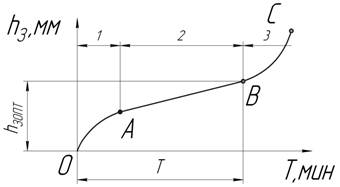
\includegraphics[width=10cm]{images/iznos.jpg}
	}
	\caption{График износа режущего инструмента в зависимости от времени его работы}\label{fig:iznos}
\end{figure}

Таким образом, показатель производительности только из-за этого фактора будет нелинейно снижаться со временем. Однако, в данной диссертационной работе стоит ограничиться гипотетическим расчётом производительности без учета динамики производства.

Разумеется, картина производственного процесса зачастую далека от идеальной. На итоговый результат влияет очень много различных условий, так или иначе снижающие эффективность производственных процессов. С 2016 года в России действует ГОСТ Р 57330-2016 <<Системы промышленной автоматизации и интеграция. Системы технического обслуживания и ремонта. Ключевые показатели эффективности>>, где показатели эффективности подразделяются на три группы: экономические, технические и организационные. Подобное справедливо и для коэффициента производительности оборудования \cite{effectivnost}. К экономическим факторам можно отнести:

\begin{enumerate}
	\item Издержки на производство продукции, включая стоимость ресурсов, аренды и т.д.
	\item Своевременный сбыт продукции, позволяющий производить продукцию без риска заполнить складские помещения до отказа.
	\item Расходы на плановое обслуживание и ремонт, во время которых оборудование будет простаивать.
	\item Количество видов изготавливаемой продукции.
\end{enumerate}

Технические факторы, влияющие на производительность:

\begin{enumerate}
	\item Уровень автоматизации отдельных операций на оборудовании.
	\item Особенности технологического процесса, допускающие простои оборудования во время, например, переустановки заготовки, подготовки покрытий поверхностей и т.д.
	\item Уровень износа движущихся частей оборудования.
	\item Уровень необходимой точности обработки поверхностей.
	\item Габаритные размеры станка и изготавливаемых изделий.
\end{enumerate}

Организационные факторы:

\begin{enumerate}
	\item Расположение станков на производственных площадях, уровень доступности станков и сопутствующей оснастки (организация рабочего места).
	\item Организация логистики заготовок на предприятии.
	\item Уровень квалификации рабочих и операторов, занятых на оборудовании.
	\item Уровень общей культуры труда на предприятии.
\end{enumerate}

Разумеется, далеко не на все из этого можно повлиять внедрением СТЗ, повышение уровня автоматизации способно затронуть лишь техническую группу показателей эффективности. Тем не менее, это имеет немаловажное значение при подготовке производства, особенно на универсальном оборудовании.

\section{Расчёт производственной мощности трехкоординатной платформы для изделия типа печатная плата} \label{sect2_3}

\subsection{Обзорная часть} \label{ssect2_3_1}

Как уже было сказано выше, производительность сильно зависит от типа и сложности выпускаемого изделия. Чем больше в нём операций, тем большее количество простоев оборудования может возникнуть. В случае с универсальным оборудованием весь техпроцесс предполагается к реализации на одном обрабатывающем центре, что вынуждает проходить операции последовательно, шаг за шагом, без возможности распараллеливания задач. Единственное, что может сократить время обработки в данном случае --- увеличение количества одновременно обрабатываемых изделий, которое, в свою очередь, зависит от размера рабочей области станка. В качестве оборудования используется трёхкоординатная платформа, описанная в разделе \ref{sect1_5} настоящей диссертации, со сменными модулями для выполнения разных типов операций.

Одним из характерных типов изделий, производимых на описанной трехкоординатной платформе, является печатная плата. Процесс ее производства достаточно комплексный и дорогой в малых масштабах производства, поскольку требует сразу несколько видов оборудования. В качестве усредненного изделия для расчёта производительности будет рассмотрена переходная плата типа SOP14/SSOP14 с разводкой под корпус DIP-14 (рис. \cref{fig:sop14}).

\begin{figure}[ht]
	\centerfloat{
		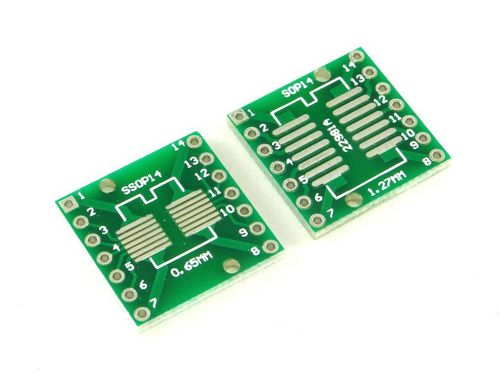
\includegraphics[width=15cm]{images/sop14.jpg}
	}
	\caption{Пример печатной платы типа SOP-14/SSOP-14}\label{fig:sop14}
\end{figure}

В первую очередь, можно определить, что при габаритных размерах платы 18 мм $\times$ 18 мм и при размерах рабочей области платформы 500 мм $\times$ 500 мм всего одновременно может обрабатываться 729 таких плат в виде цельного листа из фольгированного диэлектрика, разрезаемого потом на отдельные изделия. Плата двухсторонняя, то есть, обработке подвергаются обе поверхности с операцией переустановки в середине процесса. Плата содержит 14 проводящих отверстий по обеим сторонам от контактной площадки и 2 крепёжных отверстия, а также маркировку на обеих сторонах платы.

Всего техпроцесс насчитывает 10206 проводящих металлизированных отверстий диаметром 0,8 мм и 1458 крепёжных отверстий диаметром 2 мм, операцию печати проводящего рисунка на двух сторонах, операцию печати маркировки на двух сторонах, покрытия и финального разреза заготовки на отдельные части. Металлизация отверстий требует применения позитивного субтрактивного техпроцесса изготовления \cite{Brusnitsyna}.

\subsection{Перечень операций технологического процесса} \label{ssect2_3_2}

Далее приведен перечень операций технологического процесса производства печатной платы с нормативным временем исполнения. Операции подразделяются на установочные (У), обрабатывающие (О), контролирующие (К) и вспомогательные (В). Установочные операции напрямую связаны с размещением заготовки и инструмента, обрабатывающие --- с обработкой поверхностей, вспомогательными будут считаться все остальные.

\begingroup
	\centering
	\captionsetup[table]{skip=7pt} % смещение положения подписи
	\begin{longtable}[c]{|p{1cm}|p{11cm}|c|}
	\caption{Перечень операций}\label{tab:tp1}
	\\[-0.45\onelineskip]
	\hline
	Тип & Наименование операции & Нормативное время, с \tabularnewline \hline
		У & Установка заготовки на приспособление для сверления отверстий & 15 \tabularnewline \hline
		У & Выравнивание верхнего левого края заготовки с нулем платформы & 15 \tabularnewline \hline
		У & Установка модуля для сверления отверстий & 20 \tabularnewline \hline
		У & Установка сверла 0,8 мм & 15 \tabularnewline \hline
		В & Выравнивание оси модуля с нулевой точкой платформы & 30 \tabularnewline \hline
		О & Сверление отверстий диаметром 0,8 мм на заготовке (1 проход и переход на дальнейшую позицию по ВП с ожиданием охлаждения сверла каждые 100 проходов) & 26600 \tabularnewline \hline
		В & Переход каретки в дальнюю позицию\footnote{Позицию, максимально удалённую от нулевой точки платформы} & 5 \tabularnewline \hline
		У & Снятие заготовки с приспособления & 20 \tabularnewline \hline
		К & Визуальный осмотр отверстий & 1400 \tabularnewline \hline
		У & Снятие сверла 0,8 мм & 10 \tabularnewline \hline
		У & Установка заготовки в емкость с раствором меди & 20 \tabularnewline \hline
		О & Металлизация отверстий по методу ЭЛХМ 200\footnote{ЭЛХМ 200 --- тип химического меднения поверхностей, состоящее из пяти этапов: кондиционирования, микротравления, предварительной активации, активации и химического осаждения меди \cite{elhm200}} & 2100 \tabularnewline \hline
		У & Выемка заготовки & 10 \tabularnewline \hline
		В & Сушка заготовки & 60 \tabularnewline \hline
		К & Визуальный осмотр отверстий & 1400 \tabularnewline \hline
		У & Установка заготовки на приспособление для сверления отверстий & 15 \tabularnewline \hline
		У & Выравнивание верхнего левого края заготовки с нулем платформы & 15 \tabularnewline \hline
		У & Установка сверла 2 мм & 15 \tabularnewline \hline
		В & Выравнивание оси модуля с нулевой точкой платформы & 30 \tabularnewline \hline
		О & Сверление крепежных отверстий диаметром 2 мм на заготовке (1 проход и переход на дальнейшую позицию по УП с ожиданием охлаждения сверла каждые 100 проходов) & 3800 \tabularnewline \hline
		К & Визуальный осмотр отверстий & 700 \tabularnewline \hline
		У & Снятие сверла 2 мм & 10 \tabularnewline \hline
		У & Снятие модуля для сверления отверстий & 15 \tabularnewline \hline
		У & Переустановка заготовки с приспособления на рабочую область платформы & 20 \tabularnewline \hline
		В & Подготовка поверхности под сухой пленочный фоторезист (СПФ) & 10 \tabularnewline \hline
		В & Накрытие заготовки маской 1 (лицевая сторона) с отверстиями для фоторезиста & 10 \tabularnewline \hline
		О & Нанесение СПФ на поверхность заготовки & 60 \tabularnewline \hline
		В & Снятие маски 1 с заготовки & 10 \tabularnewline \hline
		У & Установка модуля для термической обработки фоторезиста & 20 \tabularnewline \hline
		О & Проход модуля над всей поверхностью заготовки & 120 \tabularnewline \hline
		В & Переход модуля в дальнюю позицию & 5 \tabularnewline \hline
		У & Смена модуля на УФ-лампу & 20 \tabularnewline \hline
		О & Проходы УФ-лампы над заготовкой, 16 областей по 1 минуте на 10 проходов & 9700 \tabularnewline \hline
		В & Переход каретки в дальнюю позицию & 5 \tabularnewline \hline
		У & Снятие модуля УФ-лампы & 10 \tabularnewline \hline
		К & Визуальный осмотр поверхности & 300 \tabularnewline \hline
		У & Снятие заготовки с рабочей области платформы & 15 \tabularnewline \hline
		У & Размещение заготовки в ванне с раствором кальцинированной соды & 15 \tabularnewline \hline
		О & Травление фоторезиста & 700 \tabularnewline \hline
		В & Сушка заготовки & 60 \tabularnewline \hline
		К & Визуальный осмотр поверхности & 300 \tabularnewline \hline
		У & Установка заготовки готовой стороной вверх на рабочую область платформы & 15 \tabularnewline \hline
		У & Установка защитного слоя полимера на готовую сторону заготовки & 60 \tabularnewline \hline
		У & Переворот заготовки на другую сторону & 20 \tabularnewline \hline
		В & Подготовка поверхности под СПФ & 10 \tabularnewline \hline
		В & Накрытие заготовки маской 2 (сторона с разводкой) с отверстиями для фоторезиста & 10 \tabularnewline \hline
		О & Нанесение СПФ на поверхность заготовки & 60 \tabularnewline \hline
		В & Снятие маски 2 с заготовки & 10 \tabularnewline \hline
		У & Установка модуля для термической обработки фоторезиста & 20 \tabularnewline \hline
		О & Проход каретки над всей поверхностью заготовки & 120 \tabularnewline \hline
		В & Переход каретки в дальнюю позицию & 5 \tabularnewline \hline
		У & Смена модуля на УФ-лампу & 15 \tabularnewline \hline
		О & Проходы УФ-лампы над заготовкой, 16 областей по 1 минуте на 10 проходов & 9700 \tabularnewline \hline
		В & Переход каретки в дальнюю позицию & 5 \tabularnewline \hline
		К & Визуальный осмотр поверхности & 300 \tabularnewline \hline
		У & Снятие модуля УФ-лампы & 15 \tabularnewline \hline
		У & Снятие заготовки с рабочей области платформы & 20 \tabularnewline \hline
		У & Размещение заготовки в ванне с раствором кальцинированной соды & 15 \tabularnewline \hline
		О & Травление фоторезиста & 700 \tabularnewline \hline
		В & Сушка заготовки & 60 \tabularnewline \hline
		К & Визуальный осмотр поверхности & 300 \tabularnewline \hline
		У & Установка заготовки стороной с защитным покрытием вверх на рабочую область платформы & 15 \tabularnewline \hline
		В & Выравнивание верхнего левого края заготовки с нулем платформы & 15 \tabularnewline \hline
		В & Снятие защитного покрытия & 10 \tabularnewline \hline
		У & Установка модуля для нанесения маркировки на заготовку & 20 \tabularnewline \hline
		В & Выравнивание оси модуля с нулевой точкой платформы & 15 \tabularnewline \hline
		О & Нанесение маркировки на сторону 1 (SAP-14) заготовки & 11000 \tabularnewline \hline
		В & Сушка поверхности & 30 \tabularnewline \hline
		К & Визуальный осмотр поверхности & 60 \tabularnewline \hline
		В & Переход каретки в дальнюю позицию & 5 \tabularnewline \hline
		У & Переворот заготовки на другую сторону & 15 \tabularnewline \hline
		У & Выравнивание верхнего левого края заготовки с нулем платформы & 15 \tabularnewline \hline
		В & Сброс модуля в нулевую позицию & 5 \tabularnewline \hline
		О & Нанесение маркировки на сторону 2 (SSAP-14) заготовки & 11000 \tabularnewline \hline
		В & Сушка поверхности & 30 \tabularnewline \hline
		К & Визуальный осмотр поверхности & 60 \tabularnewline \hline
		В & Переход каретки в дальнюю позицию & 5 \tabularnewline \hline
		О & Нанесение паяльной маски на сторону 2 & 30 \tabularnewline \hline
		У & Переворот заготовки на другую сторону & 15 \tabularnewline \hline
		О & Нанесение паяльной маски на сторону 1 & 30 \tabularnewline \hline
		У & Установка модуля для нанесения финишного покрытия & 30 \tabularnewline \hline
		В & Выравнивание оси модуля с нулевой точкой платформы & 30 \tabularnewline \hline
		О & Нанесение финишного покрытия на контактные площадки заготовки & 3650 \tabularnewline \hline
		В & Сушка поверхности & 30 \tabularnewline \hline
		К & Визуальный осмотр поверхности & 120 \tabularnewline \hline
		У & Переворот заготовки на другую сторону & 15 \tabularnewline \hline
		У & Выравнивание верхнего левого края заготовки с нулем платформы & 15 \tabularnewline \hline
		В & Сброс модуля в нулевую позицию & 5 \tabularnewline \hline
		О & Нанесение финишного покрытия на контактные площадки заготовки & 3650 \tabularnewline \hline
		В & Сушка поверхности & 30 \tabularnewline \hline
		К & Визуальный осмотр поверхности & 120 \tabularnewline \hline
		В & Переход каретки в дальнюю позицию & 5 \tabularnewline \hline
		У & Установка модуля с отрезной фрезой & 15 \tabularnewline \hline
		В & Выравнивание оси модуля с нулевой точкой платформы & 15 \tabularnewline \hline
		О & Разрез заготовки на отдельные изделия & 160 \tabularnewline \hline
		В & Переход каретки в дальнюю позицию & 5 \tabularnewline \hline
		У & Снятие изделий с рабочей области & 40 \tabularnewline \hline
		К & Выборочное тестирование 50 образцов из партии и контроль (5 минут на образец) & 15000 \tabularnewline \hline
		В & Упаковка изделий & 600 \tabularnewline \hline
		В & Переналадка оборудования & 300 \tabularnewline \hline
		- & \textbf{Итоговое нормативное время} & \textbf{105450} \tabularnewline \hline
	\end{longtable}
\endgroup

Таким образом, описанный технологический процесс изготовления партии печатных плат насчитывает 100 операций, из них 37 установочных, 33 вспомогательных, 18 обрабатывающих и 12 контролирующих. Итоговое нормативное время изготовления партии из 729 печатных плат составляет 105450 секунд или приблизительно 29,2 часа. Таким образом, можно утверждать, что при текущем технологическом процессе установка способна выдавать 24,9 печатных плат в час. Однако, можно отметить, что не всё нормативное время установка выполняет какие-либо операции.

Если подсчитать время работы установки, то есть, суммарное время обрабатывающих операций, то оно составит 81620 секунд или 22,6 часа. По отношению к общему времени это составляет 77,6 \%. Нетрудно заметить, что основная доля неучтённого времени приходится на промежуточные операции контроля изделий после каждого этапа обработки.

\subsection{Расчёт производительности оборудования} \label{ssect2_3_3}

Таким образом, пользуясь описанным в предыдущем разделе технологическим процессом, можно получить основные параметры, относящиеся к производительности оборудования. Параметры выработки (цикловой производительности станка) $W_o$ и трудоемкости $L$ определяются по формулам \ref{eq_2_2} и \ref{eq_2_3} \cite{web:raschet-cnc}:

\begin{equation}
W_o = \frac{V}{\Theta_w},
\label{eq_2_2}
\end{equation}

\begin{equation}
L = \frac{\Theta_w}{V},
\label{eq_2_3}
\end{equation}

где $V$ --- объем произведенной продукции в натуральном выражении, $\Theta_w$ --- время изготовления данного объема продукции. Данные параметры характеризуют производительность платформы с тех условиях, когда станок работает непрерывно, поэтому за время изготовления $\Theta_w$ принимается суммарное время обрабатывающих операций (81620 секунд). Принимая это, а также размер партии в 729 изделий, можно установить, что цикловая производительность равна 32,2 изделий в час или 0,009 изделия в секунду, а трудоёмкость --- 111,5 секунды на одну единицу продукции. Однако, данные параметры характеризуют лишь потенциальные возможности платформы.

Для выявления фактической производительности станка необходимо подсчитать коэффициент использования $\eta$. Он характеризует долю времени, затраченную на вынужденные простои станка в периоды между обрабатывающими этапами. Он рассчитывается по формуле \ref{eq_2_4}:

\begin{equation}
\eta = \frac{\Theta_w}{\Theta} = \frac{\Theta_w}{(\Theta_w + \sum \Theta_s)},
\label{eq_2_4}
\end{equation}

где $\Theta$ --- общее время производства, а $\Theta_s$ --- время простоя оборудования. Принимая ранее рассчитанные значения, получаем, что коэффициент использования равен 0,78. Таким образом, фактическая производительность оборудования $W_f$ должна вычисляться с учетом коэффициента использования:

\begin{equation}
W_f = W_o \cdot \eta = \eta (\frac{V}{\Theta_w}),
\label{eq_2_5}
\end{equation}

Итого, фактическая производительность платформы составляет 24,8 единиц продукции в час.

Простои оборудования, как правило, можно представить в виде суммы из трех составляющих (\ref{eq_2_6}):

\begin{equation}
\sum \Theta_s = \sum \Theta_r + \sum \Theta_t + \sum \Theta_o,
\label{eq_2_6}
\end{equation}

где $\Theta_r$ --- простои из-за переналадки оборудования после каждого этапа обработки, $\Theta_t$ --- простои, вызванные техническими возможностями самого станка и техпроцесса, $\Theta_o$ --- простои, вызванные не зависящими от технологического процесса внешними факторами, в том числе разного рода форс-мажорами.

Таким образом, коэффициент использования $\eta$ представляется как произведение трех более конкретизированных факторов, отражающих разные виды простоев (\ref{eq_2_7}):

\begin{equation}
\eta = \eta_r \cdot \eta_t \cdot \eta_o,
\label{eq_2_7}
\end{equation}

Коэффициент технического использования $\eta_t$ здесь играет определяющую роль и расчитывается как (\ref{eq_2_8}):

\begin{equation}
\eta_t = \frac{\Theta_w}{\Theta_w + \sum \Theta_s} = \frac{1}{1+ \sum \Theta_s / \Theta_w},
\label{eq_2_8}
\end{equation}

К техническим операциям относятся все операции за вычетом межциклового переналадочного времени, а также времени на смену модулей и их подготовку к работе. Суммарно операции, относящиеся к техническим простоям, занимают 23110 секунд. Подставив соответствующие значения, получим, что $\eta_t$ будет равен 0,779 или 78 \%. То есть, в тех случаях, когда не требуется переналадка, а рабочее место снабжено всем необходимым для работы, станок 22 \% всего времени будет простаивать.

Коэффициент переналадок $\eta_r$ отражает долю времени, когда станок простаивает в ожидании переналадки. Он рассчитывается как (\ref{eq_2_9}):

\begin{equation}
\eta_r = \frac{1}{1 + \frac{\sum \Theta_r}{\Theta_w + \sum \Theta_t}},
\label{eq_2_9}
\end{equation}

С имеющимися значениями коэффициент переналадок $\eta_r$ будет равен 99 \%, то есть, лишь 1 \% всего времени на технологический процесс будет потерян из-за переналадки оборудования.

Организационный коэффициент $\eta_o$ показывает, какую долю времени оборудование будет обеспечено всем необходимым для его работы: заготовками, инструментом, энергоресурсами и персоналом. Он рассчитывается как (\ref{eq_2_10}):

\begin{equation}
\eta_o = 1 - \frac{\sum \Theta_o}{\Theta},
\label{eq_2_10}
\end{equation}

Однако, получить данный коэффициент можно лишь в случае длительного анализа работы оборудования. При рассмотрении гипотетического случая $\Theta_o$ будет близко к 0, а коэффициент $\eta_o$, соответственно, равен 1.

Простои оборудования, приходящиеся на одну деталь (\ref{eq_2_11}):

\begin{equation}
t_d = \frac{\sum \Theta_s}{N},
\label{eq_2_11}
\end{equation}

где $N$ --- количество деталей в партии. Для описанного технологического процесса данный параметр равен 32,69 сек/деталь или 0,54 мин/деталь.

\section{Пути повышения производительности описываемого технологического процесса} \label{sect2_4}

\subsection{Возможные меры по сокращению суммарного времени производства} \label{ssect2_4_1}

Очевидно, что вышеописанный технологический процесс скован рамками одной единицы оборудования, поэтому путей повышения его эффективности не так много, как в случае с производственной линией. Порядок операций в нем строго определен технологией изготовления и его изменение ведет к нарушению оной, а следовательно, к изменениям в качестве конечного изделия. Однако, в рамках исследования можно представить несколько путей снижения суммарного времени выполнения технологического процесса путем изменения оснастки или внедрения новых технологий.

Одним из основных путей достижения более высокой эффективности является объединение операций. Методы оптимизации управляющих программ уже давно применяются в промышленности \cite{Streltsov}. Этап сверления проводящих отверстий говорит о большом количестве однотипных операций, выполнение которых занимает достаточно большое количество времени. Вопрос об одновременном сверлении отверстий поднимался ещё в 20-е годы прошлого века \cite{Efremov}, кроме того, давно известны многошпиндельные станки, позволяющие реализовать одновременную обработку отверстий в детали (рис. \cref{fig:multi-sp}). Однако, в случае трехкоординатной платформы, под одновременное сверление отверстий необходимо проектировать специализированный модуль, который будет иметь группу шпинделей со сверлами, приводящимися в движение единым двигателем. Данный модуль позволит существенно снизить время обработки в зависимости от количества шпинделей, однако, данный тип повышения производительности характеризуется затратами на проектирование соответствующего модуля, органичениями на применяемый инструмент в модуле и узкой направленностью самого модуля, не позволяющего применять его в других технологических процессах с другими требуемыми параметрами отверстий и расстояний между ними. Кроме того, в случае мелкосерийного производства такой подход нежелателен.

\begin{figure}[ht]
	\centerfloat{
		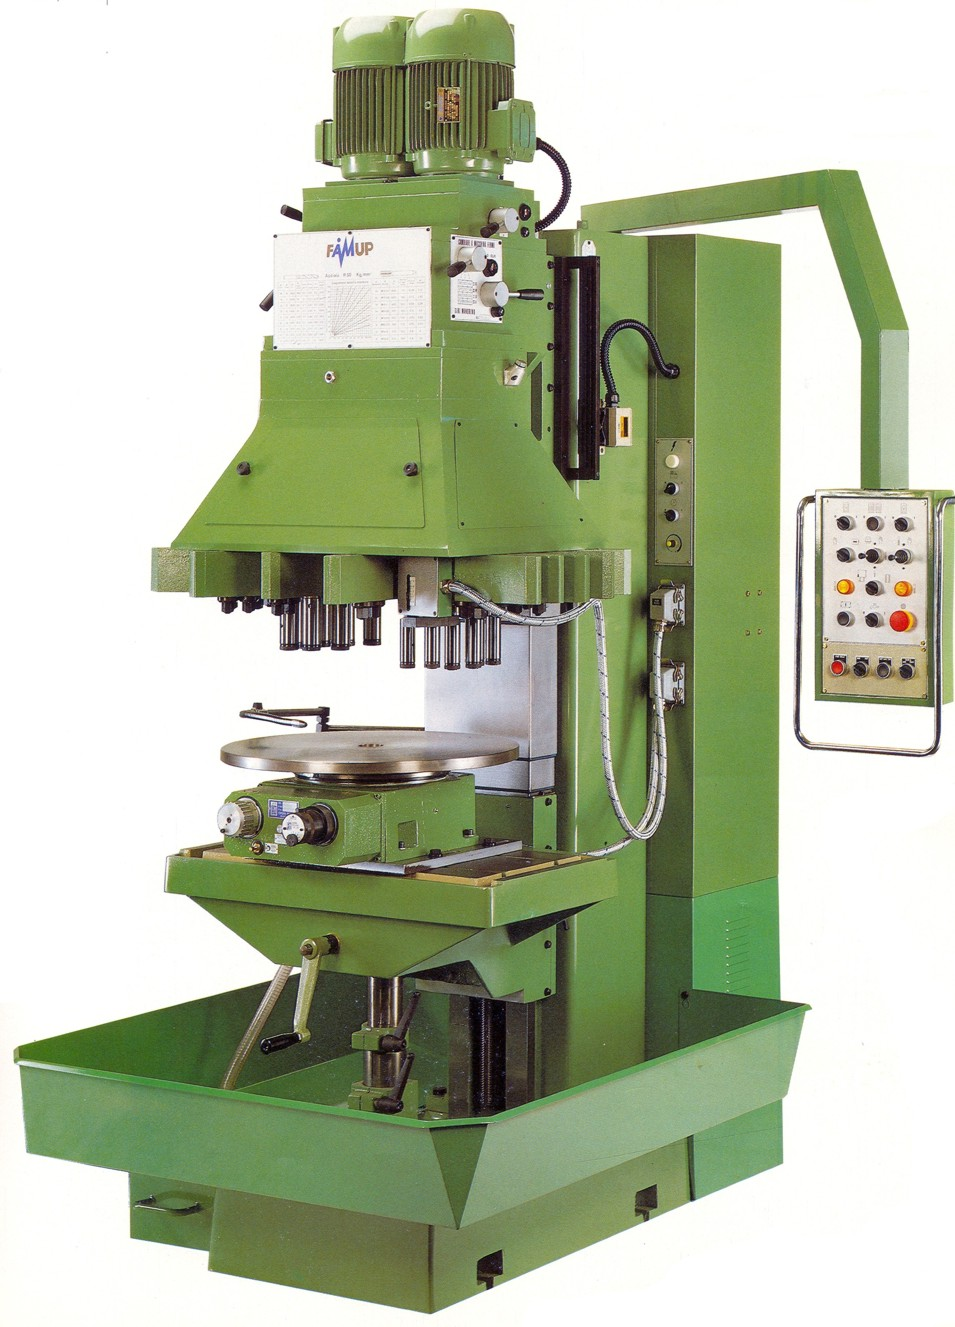
\includegraphics[width=8cm]{images/multi-sp.jpg}
	}
	\caption{Многошпиндельный сверлильный станок с ЧПУ}\label{fig:multi-sp}
\end{figure}

Другой способ оптимизации --- объединение операций, выполняющихся вне оборудования. К таковым относятся металлизация отверстий и травление фоторезиста. Данный способ направлен на группирование операций, не требующих выполнения на оборудовании и высвобождающих его для обработки другой заготовки. Но стоит отметить, что далеко не каждый техпроцесс позволяет провести соответствующую перестановку операций, и рассмотренный выше не является исключением. Металлизацию отверстий невозможно проводить после операции травления фоторезиста, а перед травлением фоторезист необходимо нанести и подготовить при помощи маски с УФ-лампой либо пробегом лазера по будущим дорожкам платы. Таким образом, данный способ оптимизации работы платформы не подходит для описанного случая.

Ещё одним возможным улучшением является смещение некоторых конечных операций на время исполнения следующего цикла обработки. Так, операции постпроизводственного контроля и упаковки можно проводить уже после начала следующего цикла, этому способствует и продолжительное время обработки большого массива отверстий под проводящие контакты. Данное смещение сократит суммарное время цикла обработки на 15600 секунд. Однако, стоит отметить, что далеко не в каждом технологическом процессе существует подходящее <<окно>> для выполнения оператором данных действий, в противном случае оператор будет отвлекаться на другие задачи, что может существенно снизить итоговое качество партии. Найм же ещё одного рабочего, который будет заниматься только данной задачей, в рамках небольшого предприятия нерационален и ведёт к дополнительным издержкам. Кроме того, даже в случае большого <<окна>> существует вероятность нештатных ситуаций, на которые будет вынужден реагировать оператор, отвлекаясь от процесса контроля готовых изделий.

Также можно упомянуть вариант с одновременной установкой двух модулей на каретку платформы по разные стороны от неё. Это позволит в некоторых случаях проводить операции параллельно (например, нанесение покрытия и его отверждение лампой) и сэкономить немного времени на установке модулей. Но стоит отметить, что второй неактивный модуль может утяжелить каретку платформы, что скажется на скоростях перемещения, также на него могут действовать нежелательные вибрации, а в отверстия и пазы забиваться пыль от работы первого модуля. Кроме того, второй модуль увеличивает габаритные размеры каретки, что может снизить площадь обрабатываемой поверхности.

\subsection{Перспективы внедрения систем технического зрения} \label{ssect2_4_2}

Вышеописанные способы оптимизации, хоть и могут быть применены в какой-то степени к вышеописанному технологическому процессу, но не являются универсальными решениями. В условиях постоянной смены выпускаемых изделий каждый анализ техпроцесса по части оптимизации может вылиться в ненужную работу, которая потеряет свою актуальность уже <<завтра>>, а со следующим изделием всё необходимо проводить заново. Каждый технологический процесс будет требовать своего подхода и то, насколько критичным там будет являться соблюдение порядка операций, выяснить невозможно \cite{Pisarevsky}.

Помимо вышеописанных способов стоит подробно рассмотреть перспективы внедрения СТЗ в систему управления платформы. Данное решение подразумевает автоматизацию нескольких типов операций, являющихся общими для разных технологических процессов, к примеру, операции контроля или выставления нуля инструмента. Разумеется, в условиях различных типов изделий потребуется выдерживать разные параметры работы СТЗ, однако конфигурация данного оборудования возможна в рамках управляющей программы перед началом цикла производства. Протоколы передачи данных позволяют удаленно конфигурировать не только контроллеры обработки данных, но и сами камеры.

Как уже отмечалось в первой главе данной диссертации, СТЗ широко применяется в задачах контроля и наблюдения. Операции контроля в описанном техпроцессе --- это то, что сократится с внедрением СТЗ в первую очередь. Современные возможности камер и обрабатывающего оборудования позволят контролировать целостность и ровность дорожек, непротрав фоторезиста, форму отверстий. В контролирующих операциях, в основном, применяется метод сравнения с эталоном, позволяющий упростить синтез алгоритмов. Сюда же можно отнести и измерительную функцию, при помощи которой будет определяться расположение отверстий по отношению к углу заготовки и друг к другу. Однако, следует заметить, что измерительная функция СТЗ должна быть обеспечена соответствующими метрологическими мероприятиями.

Применение СТЗ также может упростить установку и соотнесение систем координат платформы, что сократит время на выставление инструмента в начальную позицию. Очевидно, что модули могут сильно различаться между собой, поэтому СТЗ должна будет выполнять операцию идентификации модуля по некоему признаку или метке. 

Также при помощи СТЗ можно осуществлять контроль процесса обработки заготовки, например, контроль расположения заготовки для избежания ситуаций ее смещения относительно нужной позиции. Это снизит как вероятность сбоев в процессе работы платформы, так и предотвратит возможную порчу оборудования и инструмента.

Данные функции составляют далеко не полный перечень возможностей СТЗ в промышленном производстве. Вышеописанные преимущества внедрения СТЗ будут описаны в данной диссертации далее.

\section{Выводы по второй главе} \label{sect2_5}

В данном разделе были рассмотрены вопросы производительности оборудования. Как одна из определяющих характеристик производства, методы расчета и оптимизации сильно зависят как от типа выпускаемых изделий, так и от организации производства. На текущий момент оборудование с ЧПУ не используется эффективно, поэтому вопросы совершенствования технологий важны для организации высокотехнологичного производства. В подразделе рассмотрены наиболее вероятные причины потерь времени работы оборудования в разных областях возникновения, а также факторы, внутренние и внешние, которые в итоге ведут к снижению эффективности производства.

Был рассмотрен технологический процесс типового изделия, который можно производить на описанной в разделе \ref{sect1_5} трехкоординатной платформе. Проведен обзор выпускаемого изделия, необходимые для его производства технологии. Представлен перечень операций производства партии двухсторонних переходных печатных плат типа SAP-14/SSAP-14 с нормативным временем каждой операции.

На основе рассмотренного технологического процесса был произведен расчёт различных параметров производительности описанной трехкоординатной платформы с ЧПУ. Данный расчёт показал, что с данных изделием и в гипотетическом плане установка работает с эффективностью в 78 \%, однако, данный показатель может измениться в долгой перспективе вследствие износа оборудования, сбоев и форс-мажоров.

Далее описанный технологический процесс был проанализирован на предмет возможного сокращения времени обработки изделия. Был предложен ряд мер, каждая из которых так или иначе не имеет рационального применения в условиях мелкосерийного производства. Особый интерес вызывает внедрение в техпроцесс системы технического зрения. Более подробно данный вопрос будет рассмотрен в следующих главах данной диссертации.